\section{Why Photovoltaic}

 \paragraph{Abundance} The total solar irradiance hitting the outer Earth atmosphere is around \SI{1361}{\watt\per\square\metre},\cite{Kopp2011} which, considering our planet cross section area, makes \SI{1.6e17}{\watt}.
 Nature conveys this energy in plenty of ways, including the generation of every renewable and most of non-renewable energy sources.
 Solar energy is effectively the primary energy source for our planet's ecosystem, so it's the most interesting source of energy for human usage.

 \paragraph{Availability} Its ubiquitous availability can be the leverage for some degree of economical power levelling across different regions of the planet.
 This is even more interesting when considering that most of the regions where life quality is seriously affected by economy (represented in Fig.~\ref{fig:world_map-HDI} by the Human Development Index) have abundance of solar irradiation (represented in Fig.~\ref{fig:world_map-PVOUT} by the ratio between the photovoltaic electric energy that can be obtained over the nominal power of an installed solar panel).

\begin{figure}%[!hbtp]%
        \centering
        \begin{subfigure}[b]{1\textwidth}
                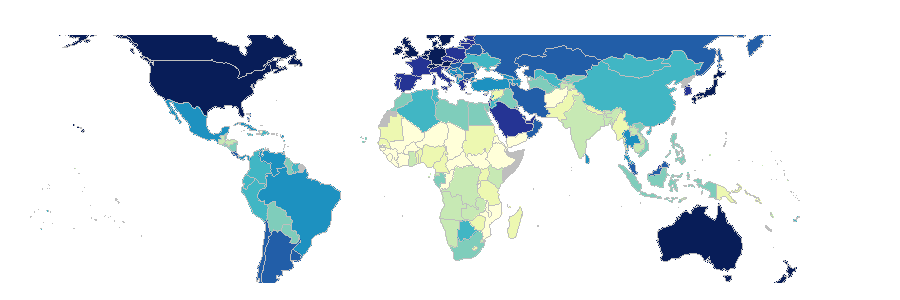
\includegraphics[width=1\textwidth]{world_map-HDI/world_map-HDI.pdf}
                \subcaption{Human development index by region}\label{fig:world_map-HDI}
        \end{subfigure}
        
        \begin{subfigure}[b]{1\textwidth}
                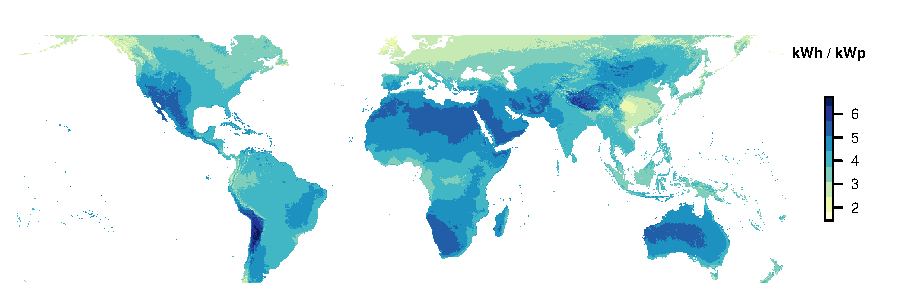
\includegraphics[width=1\textwidth]{world_map-PVOUT/world_map-PVOUT.pdf}
                \subcaption{Daily photovoltaic electricity potential}\label{fig:world_map-PVOUT}
        \end{subfigure}
    
        \begin{subfigure}[b]{1\textwidth}
    		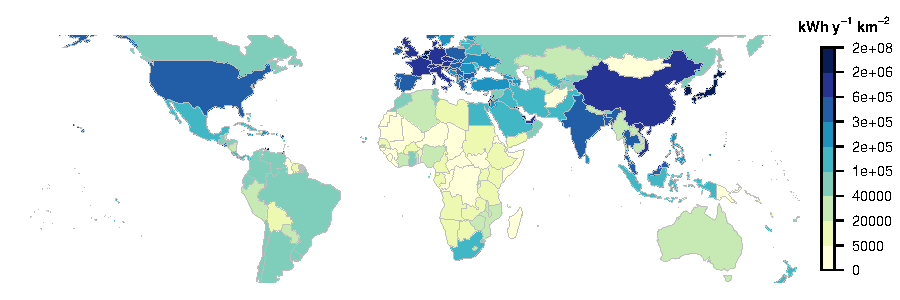
\includegraphics[width=1\textwidth]{world_map-electrical_vs_land/world_map-electrical_vs_land.pdf}
    		\subcaption{Yearly electricity consumption over region land area}\label{fig:world_map-electrical_vs_land}
    	\end{subfigure}
        \caption{Data in (\textbf{a}) represent the human development index: 
        	"a summary measure of average achievement in key dimensions of human development: a long and healthy life, being knowledgeable and have a decent standard of living"
        	from UNDP\cite{UNDP2018} (missing data in grey); data in (\textbf{b}) represents the photovoltaic electricity potential: considering a photovoltaic module installed in a region, is the ratio between the average daily produced energy, in kWh, and the nominal power, or nameplate capacity, of the installed module;\cite{Solargis2018} data in (\textbf{c}) represents the yearly electricity consumption\cite{CIAa} (comparing total electricity generated annually plus imports and minus exports) on a country scale divided by country land surface,\cite{CIA} expressed in kilowatt-hours per year per square kilometre.}\label{fig:world_map}
\end{figure}

 \paragraph{Resilience} Photovoltaic is the electric energy production method that best matches a distributed and decentralized network model, with the only single-point-of-failure being the climate variability.
 Combined with accumulation (needed for night time usage) and with other energy sources, it can be the pivot of a completely resilient electric energy provisioning system.

 \paragraph{More energy is not enough} It is intuitive that increasing the energy production is a high-price solution to the growing energetic demand.
 Indeed, in some regions a decrease in the electricity consumption has to be included for a long-term solution.
 For example, a study\cite{Margolis2016} reports that if every rooftop (not considering utility-scale solar facilities) in United States of America was covered with solar panel, just the 39~\% of its nowadays national consumption would be covered.
 In Fig.~\ref{fig:world_map-electrical_vs_land} we can see how electricity consumption density is greatly inhomogeneous and comparing with the photovoltaic potential map in Fig.~\ref{fig:world_map-PVOUT}, it is evident that such a problem is shared with many other poorly insulated but energy eager regions.
 Both an increase in machinery's efficiency and a change in life-style can be part of the solution, following the example and thinking at life-style, in USA the per capita energy usage is more than twice the European average, and five times the Latin America average.\cite{IEA}
 
 \paragraph{And more research is needed} Every source of electrical energy we can think of works via the conversion of motive power (a flow of steam, wind, or water, waves, tides...) to electricity, which relays on the well established electric generator. Except photovoltaic energy. This very simple difference already hints for the huge step in technology required by photovoltaics as compared to other energy sources.

\section{PhotoVoltaic Effect}

 \paragraph{Light absorption} 

 \paragraph{Exciton generation} 
 
 \paragraph{Exciton splitting} 
 
 \paragraph{Charge drift and charge diffusion} 
 
 \paragraph{Charge collection} 
 
 \paragraph{Electromotive force} 

\section{Perovskite Solar Cells}

 \paragraph{Electromotive force} 

 \paragraph{Electromotive force} 

\section{Efficiency Limiting Factors}

 \paragraph{Charge recombination types} 

\section{Studying and Understanding the System}

\section{Aims}